\documentclass[12pt,a4paper]{article}
\usepackage{geometry}
\usepackage{hyperref}
\usepackage{longtable}
\usepackage{enumitem}
\usepackage{titlesec}
\usepackage{graphicx}

\geometry{margin=1in}
\setlist{nosep}

\title{Liberty File Analyzer and Merger \\ \large User and Developer Documentation}
\author{Project Team}
\date{\today}

\begin{document}
\maketitle
\tableofcontents
\newpage

% -----------------------------
\section{Introduction}
This document provides complete documentation for the Liberty File Analyzer and Merger tool. The software allows engineers to:
\begin{itemize}
    \item Parse Liberty \texttt{.lib} files into structured representations.
    \item Analyze cell, pin, timing, and power data.
    \item Merge multiple libraries or multiple cells into a consolidated output.
    \item Interact easily through a graphical user interface (GUI).
\end{itemize}

The tool is written in Python and is intended for VLSI/ASIC designers working with Liberty format files.

\section{Installation}
\begin{enumerate}
    \item Clone the repository:
    \begin{verbatim}
    git clone https://www.github.com/xiayu87/mrglib
    cd mrglib
    \end{verbatim}
    \item Install dependencies:
    \begin{verbatim}
    pip install -r requirements.txt
    \end{verbatim}
    \item Run the GUI application:
    \begin{verbatim}
    python gui_app.py
    \end{verbatim}
\end{enumerate}

\section{Graphical User Interface (GUI)}

The GUI provides the primary way to interact with the tool. It was implemented in \texttt{gui\_app.py}.

\subsection{Main Features}
\begin{description}
    \item[Load Library] Opens a file dialog to select one or more Liberty files.
    \item[Analyze] Parses the selected file(s) and displays structured information on cells, pins, timing, and power.
    \item[Merge] Combines multiple Liberty files (or multiple cells) into a unified library.
    \item[Export] Saves the analyzed or merged result into a new file (\texttt{merged.lib}).
    \item[Logs/Output] Shows status messages and error feedback.
\end{description}

\subsection{Buttons and Parameters}
Each button in the GUI has a dedicated function:
\begin{longtable}{p{0.25\linewidth}p{0.7\linewidth}}
\textbf{Button} & \textbf{Functionality} \\ \hline
Load File(s) & Opens dialog to choose Liberty files. Multiple selection allowed. \\
Analyze & Runs parser on loaded files, producing a detailed structural view. \\
Merge & Combines loaded files into a new internal representation. \\
Export & Writes out the merged structure into a valid \texttt{.lib}. \\
Exit & Closes the application gracefully. \\
\end{longtable}

\newpage
\section{Configuration Files}
The tool allows customization through both \texttt{config.py} and \texttt{config.yaml}.

\subsection{Important Parameters}
\begin{description}
    \item[postfix.regex] Regular expression used to detect postfixes in cell names.
    \item[precedence] Rules for resolving duplicate attributes (e.g., ``first'' or ``later'').
    \item[units\_policy] Defines which units to adopt when conflicts exist (options: ``first'', ``later'').
    \item[rewrite\_attr\_equals\_cellname] Boolean option; if true, rewrites internal attributes to match the cell name.
\end{description}

\subsection{Editing Config}
Both YAML and Python formats are supported. The YAML file is preferred for non-developers.

\section{Module Documentation}

\subsection{parser.py}
\begin{itemize}
    \item Reads Liberty \texttt{.lib} files.
    \item Builds structured dictionaries for cells, pins, timing, and power.
    \item Provides error checking for malformed syntax.
\end{itemize}

\subsection{merger.py}
\begin{itemize}
    \item Combines multiple parsed Liberty files into one structure.
    \item Ensures no duplicate cell names.
    \item Resolves conflicts using precedence rules from configuration.
\end{itemize}

\subsection{analyze.py}
\begin{itemize}
    \item Inspects parsed library objects.
    \item Produces summary tables of cells, pins, timing arcs, and power entries.
\end{itemize}

\subsection{serializer.py}
\begin{itemize}
    \item Converts internal data structures back into valid Liberty syntax.
    \item Handles formatting, indentation, and attribute ordering.
\end{itemize}

\subsection{util.py}
\begin{itemize}
    \item Contains helper functions for string manipulation, regex matching, and validation.
\end{itemize}

\subsection{config.py}
\begin{itemize}
    \item Provides default configuration values (used if YAML not present).
\end{itemize}

\subsection{gui\_app.py}
\begin{itemize}
    \item Implements GUI window and event bindings.
    \item Integrates all functions: parse, analyze, merge, export.
\end{itemize}

\section{Command-Line Interface (CLI)}
\textbf{Note: This section is under development.}  

The codebase contains placeholders for CLI commands such as \texttt{analyze} and \texttt{merge}, but they are not stable yet. For now, only the GUI workflow is officially supported.

\section{Output Files}
\subsection{Analyzed Results}
Displayed in GUI and optionally saved as structured JSON.

\subsection{Merged Library}
Produced as \texttt{merged.lib}, guaranteed to follow Liberty format.

\section{Error Handling}
Common issues:
\begin{itemize}
    \item \textbf{Malformed input:} Parser will log a warning and skip invalid blocks.
    \item \textbf{Conflicting attributes:} Resolved using precedence rules.
    \item \textbf{Empty merge:} If input libraries share no compatible cells, merged output may be empty.
\end{itemize}

\section{Tutorial}
Following is a step by step tutorial to merge cells in a library. 

\subsection{Main Window}
The GUI provides a visual interface for interacting with Liberty files. Users can load input files, analyze them, merge cells, and export results.

\begin{figure}[h]
\centering
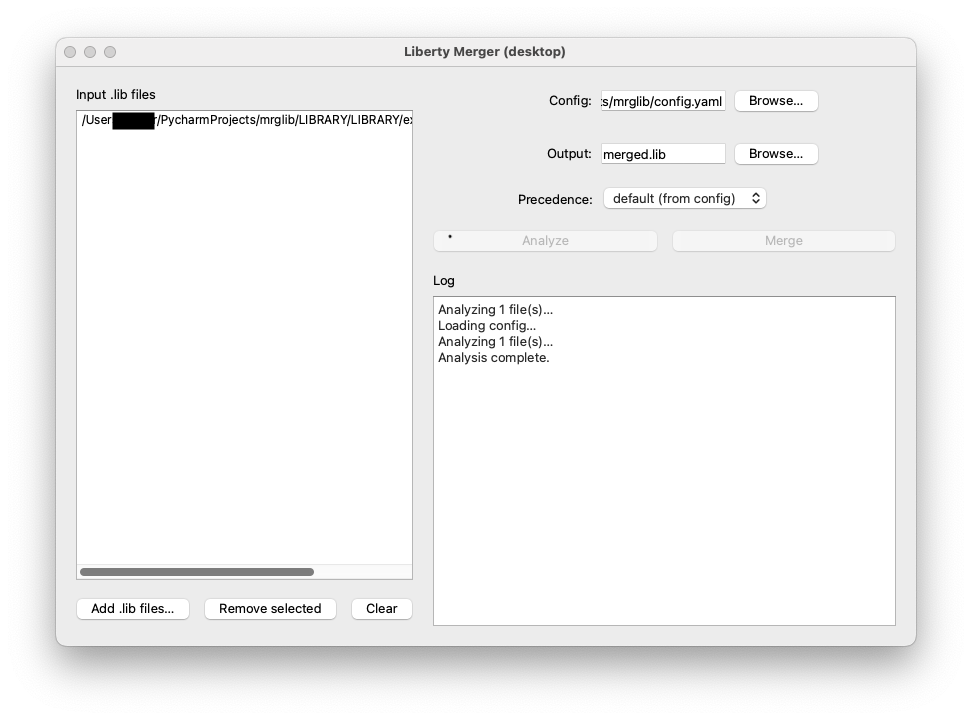
\includegraphics[width=0.9\textwidth]{1.png}
\caption{Main GUI window on launch.}
\end{figure}

\subsection{Loading Input Files}
The user can select one or multiple Liberty files for parsing. The selected files are listed in the interface for further processing.

\begin{figure}[h]
\centering
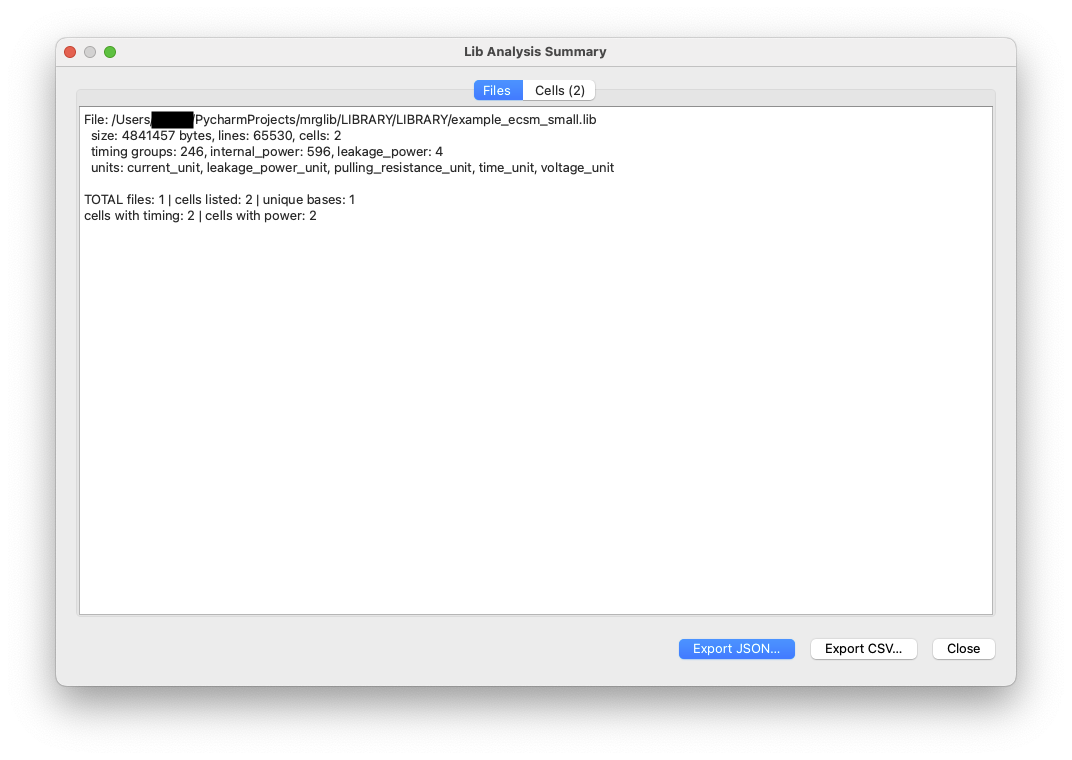
\includegraphics[width=0.9\textwidth]{2.png}
\caption{File selection dialog for Liberty files.}
\end{figure}

\subsection{Analysis}
The \textbf{Analyze} button triggers the analysis of selected files. This checks syntax validity, cell completeness, and reports errors.

\begin{figure}[h]
\centering
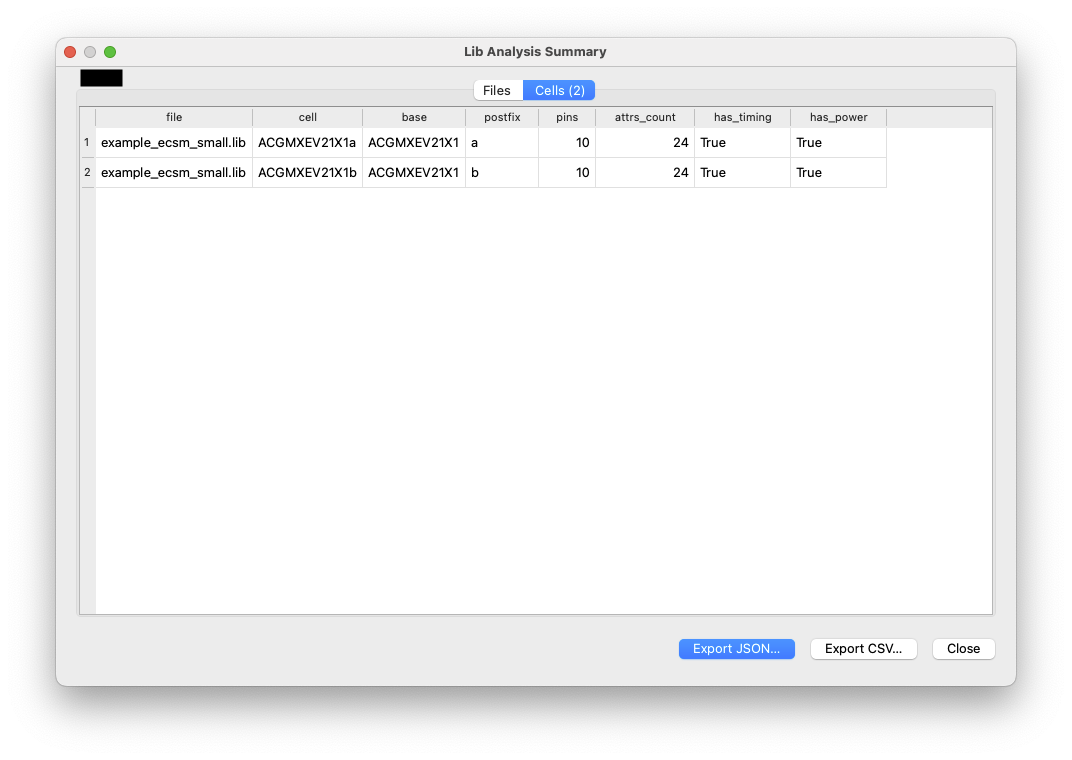
\includegraphics[width=0.9\textwidth]{3.png}
\caption{Analysis results displayed in GUI.}
\end{figure}

\subsection{Merging Cells}
The \textbf{Merge} button allows merging multiple cells across files, or merging subcells within a single file. The merged result is displayed in a text area.

\begin{figure}[h]
\centering
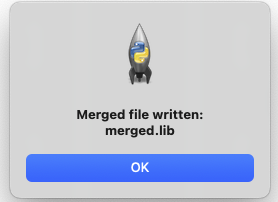
\includegraphics[width=0.9\textwidth]{4.png}
\caption{Merged cells preview in GUI.}
\end{figure}

\subsection{Exporting Results}
The \textbf{Export} button saves the merged Liberty file into a specified directory.

\begin{figure}[h]
\centering
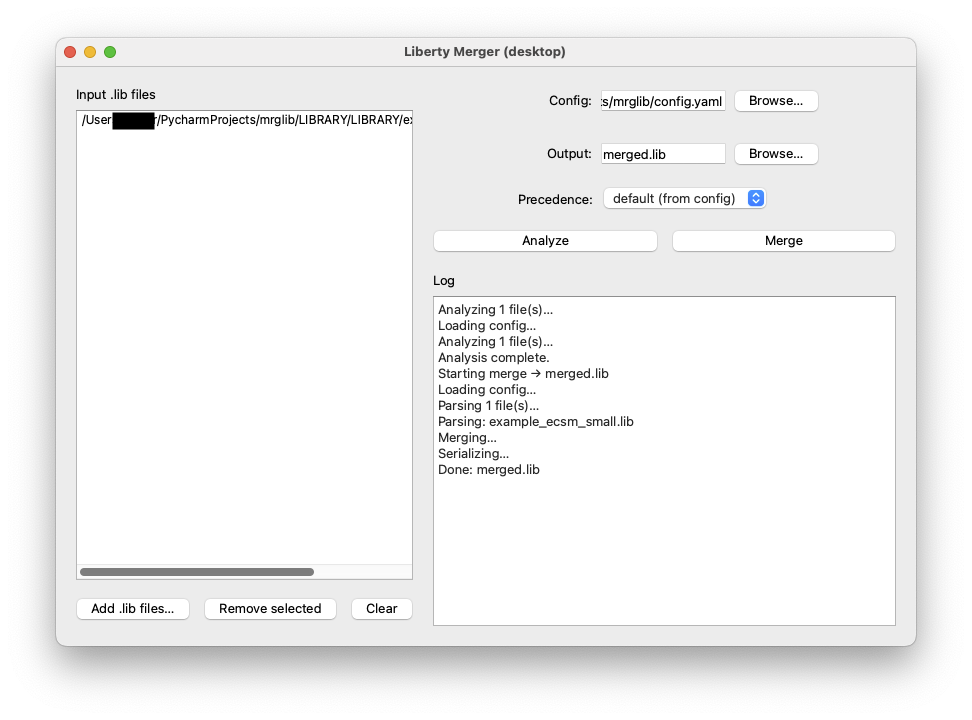
\includegraphics[width=0.9\textwidth]{5.png}
\caption{Export merged Liberty file.}
\end{figure}

\subsection{Parameter Settings}
Configuration options are available under the \textbf{Settings} menu. These include library type selection (CCS, ECSM), merge rules, and error handling preferences.

\begin{figure}[h]
\centering
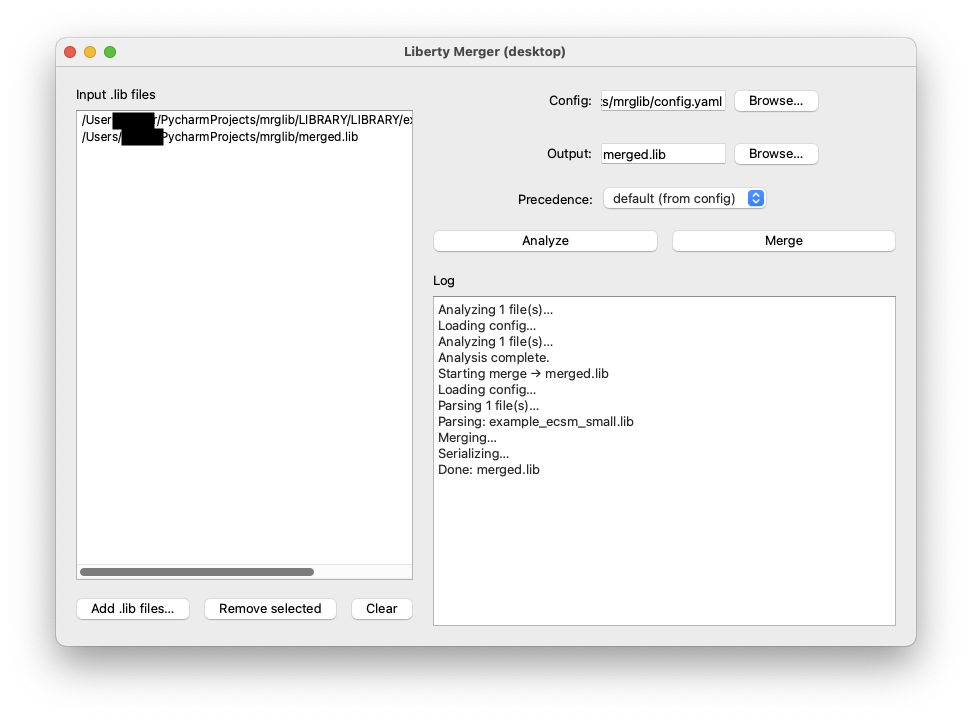
\includegraphics[width=0.9\textwidth]{6.png}
\caption{Configuration settings panel.}
\end{figure}

\subsection{Progress Monitoring}
The tool provides progress bars during heavy operations (e.g., parsing large libraries).  

\begin{figure}[h]
\centering
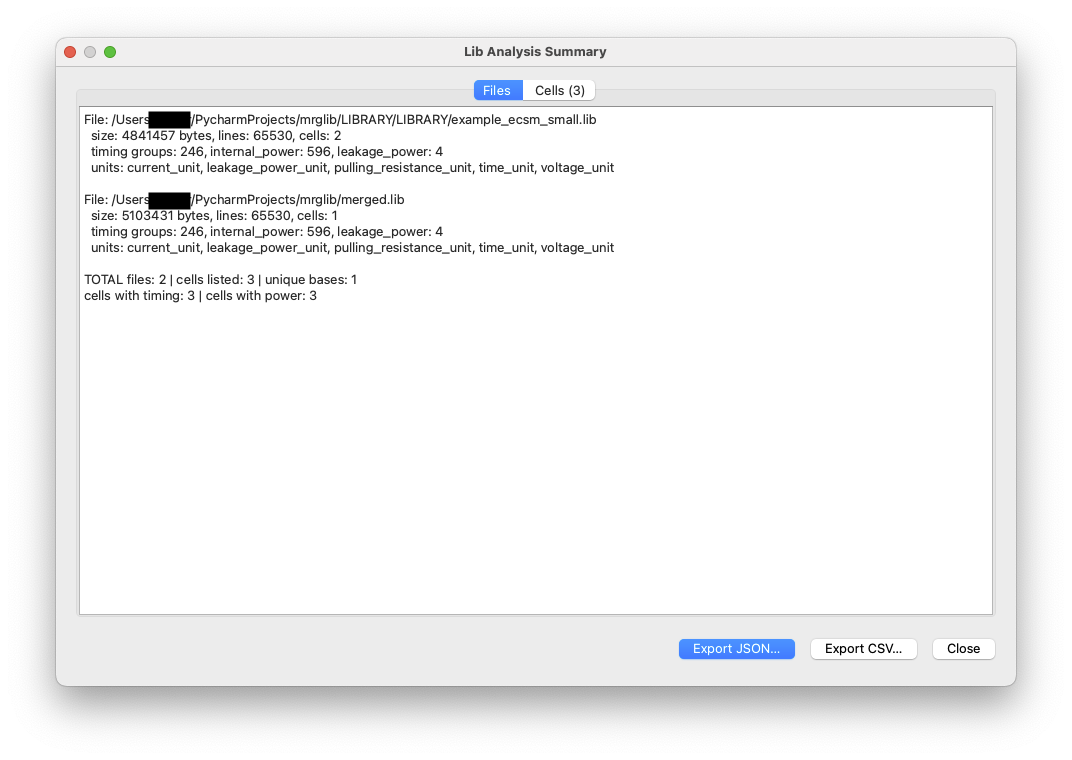
\includegraphics[width=0.9\textwidth]{7.png}
\caption{Progress monitoring during merging.}
\end{figure}

\subsection{Results Summary}
After merging, a summary panel displays statistics such as number of cells merged, timing arcs retained, and power models combined.

\begin{figure}[h]
\centering
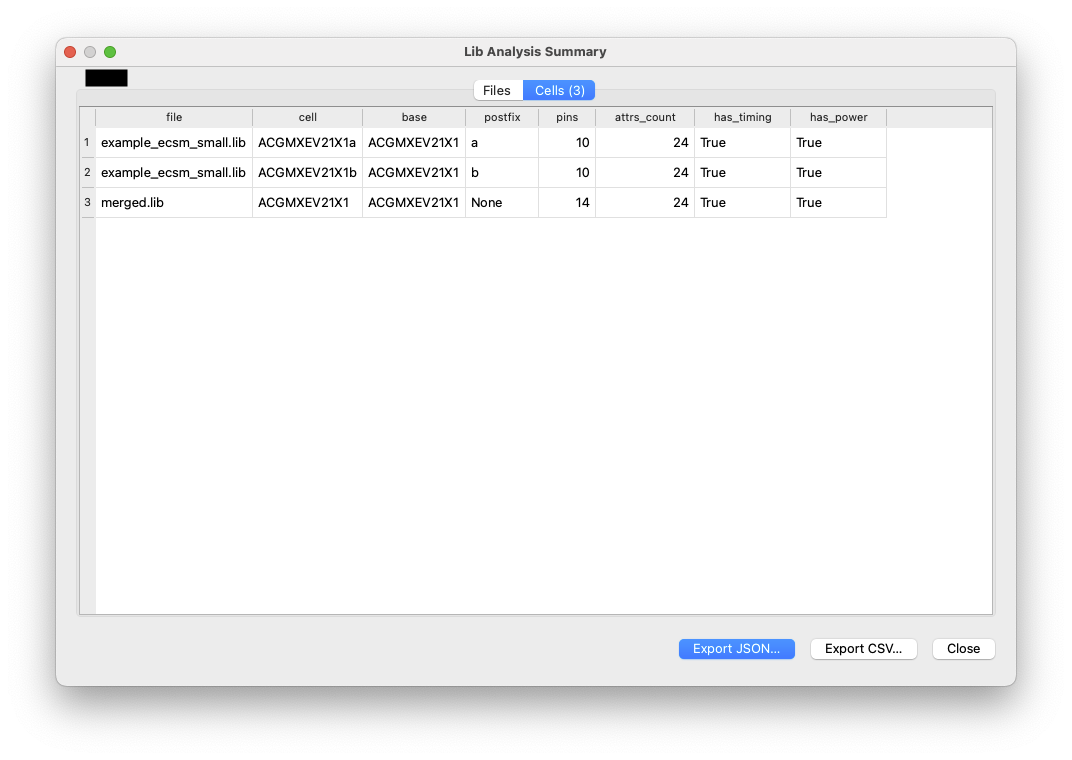
\includegraphics[width=0.9\textwidth]{8.png}
\caption{Summary of merged results.}
\end{figure}

\section{Future Work}
\begin{itemize}
    \item Complete CLI command set.
    \item Add visualization of timing/power graphs.
    \item Expand error reporting to pinpoint faulty cells.
\end{itemize}

\end{document}
